\documentclass{article}

\usepackage{times}
\usepackage{uist}

\usepackage{graphicx}
\usepackage{caption}
\usepackage{subcaption}

\usepackage{dblfloatfix} 

%\usepackage{mathptmx}
% \usepackage{graphicx}
%\usepackage{subfig}
%\usepackage{url}
%\usepackage{wrapfig}

\begin{document}

% --- Copyright notice ---
\conferenceinfo{UIST'12}{October 7-10, 2012, Cambridge, MA, USA}
\CopyrightYear{2012}
\crdata{978-1-xxxx-xxxx-x}

% Uncomment the following line to hide the copyright notice
% \toappear{}
% ------------------------

\bibliographystyle{plain}

\title{A link between physical and digital drawing \\
       through spatial augmented reality}

%%
%% Note on formatting authors at different institutions, as shown below:
%% Change width arg (currently 7cm) to parbox commands as needed to
%% accommodate widest lines, taking care not to overflow the 17.8cm line width.
%% Add or delete parboxes for additional authors at different institutions. 
%% If additional authors won't fit in one row, you can add a "\\"  at the
%% end of a parbox's closing "}" to have the next parbox start a new row.
%% Be sure NOT to put any blank lines between parbox commands!
%%

\author{
\parbox[t]{9cm}{\centering
	     {\em Jeremy Laviole}\\
   Univ. Bordeaux, LaBRI, UMR 5800, F-33400 Talence, France.\\
  CNRS, LaBRI, UMR 5800, F-33400 Talence, France.\\
   INRIA, F-33400 Talence, France.\\
	     laviole@labri.fr \vspace*{-0.4cm}}
\parbox[t]{9cm}{\centering
	     {\em Martin Hachet}\\
	     Inria, F-33400 Talence, France.\\
	     LaBRI, UMR 5800, F-33400 Talence, France.\\
	     martin.hachet@inria.fr}
}

\maketitle

\abstract

Physical drawing is being more and more replaced by digital drawing. Although the digital world offers a wide range and tools and techniques, they only allow edition of digital drawings.
In this paper, we propose some tools to link physical drawing and digital drawing through spatial augmented reality (SAR). These tools enables a wide variety of new uses of image edition software: for the creation of physical drawings and to mix drawings and projections to create light effects.                                                                                                                                                                                                                                                                                               

\classification{H5.1 [Information interfaces and presentation]:
Multimedia Information Systems. - Artificial, augmented, and virtual realities}

\terms{Design, Human Factors}

\keywords{Spatial augmented reality, user interfaces, arts, interactive projection}

\tolerance=400 
  % makes some lines with lots of white space, but 	
  % tends to prevent words from sticking out in the margin

\section{INTRODUCTION}

Software for digital creations provide a rich experience and allows a wide variety of creation styles. For many years now many papers propose advanced techniques to mimic physical drawing~\cite{VBGS08}. Conversely, improving physical drawing or painting have received less attention~\cite{flagg2006projector}. Unlike digital creation, a physical drawing is unique and may contain traces of its history.
It creates a link between the artist and the creation, this history is different with a digital drawing that can be saved at different states and always edited.
The drawing or painting can be transported, has to be taken care of, and it will age. The whole creation process requires to buy materials, and each material will provide a different experience. The smell, contact with paper and the experience to master the different tools provide a creative experience very different to the digital one. 

In this paper, we propose to use an image edition software (The Gimp~\cite{gimp2004image}) for physical artistic creations. To achieve this, the drawing is captured and sent to the drawing software. Then the user can add new elements, try some colourisation and project it on the physical drawing. This paper present some early results, and ideas on the use of existing software solutions  for physical drawings.


\section{System overview}

%\subsection{Spatial augmented reality}

The Spatial augmented reality (SAR) system is composed of a projector camera system (procam), an additional high resolution camera to capture the drawings, and a stylus input. For a detailed description of the procam system, please have a look at~\cite{laviole:2012}. It allows fast tracking of a piece of paper and precise projection on it. The tracking latency is not an issue for this kind of application, but the projection precision is the current limitation. Although high resolution cameras are relatively cheap, the current optics of the projectors are not made to project on small surfaces. The current projection precision is about 1 pixel/mm. 


\begin{figure}[tb]
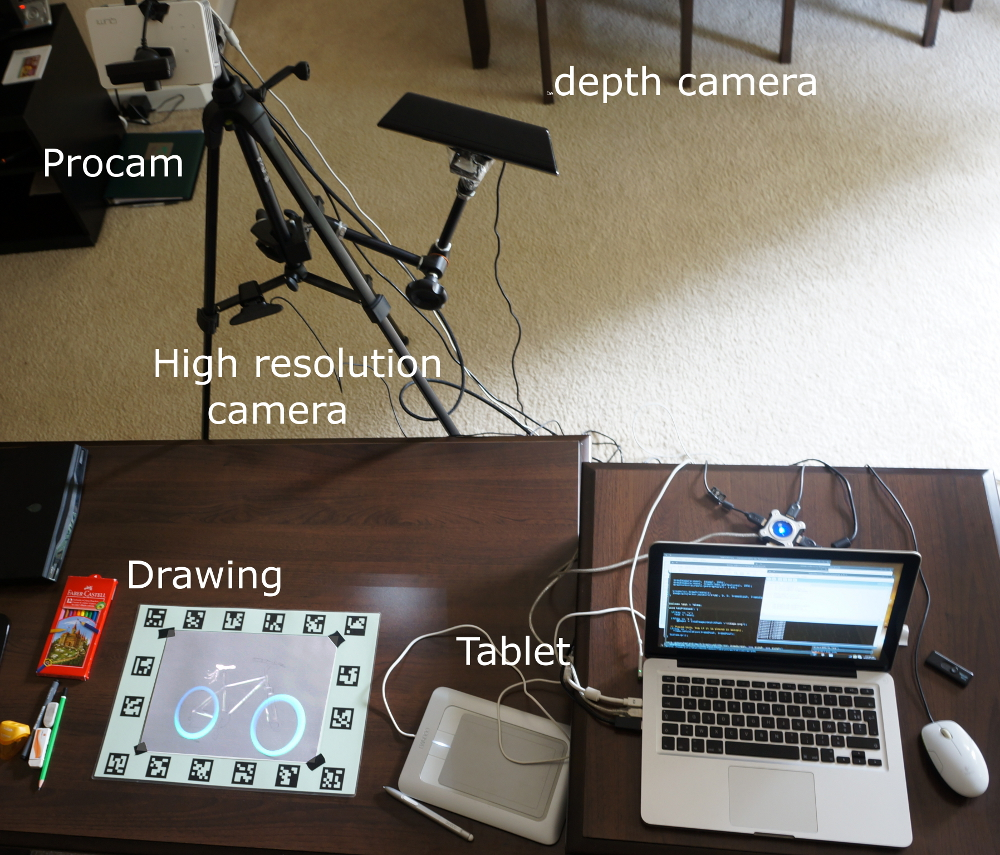
\includegraphics[width = 73mm]{DSC00299-2-rogne-annote.JPG}
\caption{Overview of the system.} 
\label{fig:setup}
\end{figure}

The transfer from the physical world to the digital world is made by a high resolution web camera. 
While drawing, the artist can add digital construction lines using the stylus and the multi-touch interface. These direct construction are directly added on the drawing, and could also be saved and sent to the drawing software.  

%Only the drawing is extracted from the image and save to the disk. (ref image ?). The image can be opened with an image edition software. In this paper we chose to use The Gimp, but any edition software can be used. Once the image is imported, a drawing layer has to be created. The edition of the drawing will be made on this layer and the projection will consist only in this layer. Once the  layer is done, the user can save this layer and hit the load button in the SAR tool. Consequently the physical drawing will contain the added digital informations.  

%In order to make the system more direct, we also included some digital drawing tools into our SAR software. Some basic elements such as line, curve and freehand drawing can be done directly. The lines and curves have control points which can be placed directly using the touch interface. The tablet device allows the user to draw digital lines onto the real drawing. In the next section, we describe how to use our system by a demonstration on a simple example. 


\section{Example use}

In this example (Figure~\ref{fig:velo6illu}), we show the firsts steps of the creation of a drawing using our system. We start by a photo (\ref{fig:bike}) projected on a paper sheet. The artist uses the projection to draw the first contours of the bike. Once it is done, the drawing is captured by a camera (\ref{fig:extract}) and the drawing is extracted (\ref{fig:gimp1}); then exported to the drawing software and added as a layer on the first image, as illustrated in Figure~(\ref{fig:gimp2}). 
In the drawing software, we decided to try different looks for the bike by selecting the texture elements from the bike and adding coloured wheels.
In the image edition software, the user can have a preview of the projection, by mixing the captured image and the new layer (\ref{fig:gimp2}). Only the new layer is projected, the result is illustrated in~(\ref{fig:proj}). From this, the user can continue the physical drawing, or add digital elements using the tablet input. Figure~\ref{fig:zoom} shows some details of the projection on the drawing, the saddle have been painted and decorated using the tablet input. 

\begin{figure}[!htb]
        \begin{subfigure}[b]{0.20\textwidth}
                \centering
                
\includegraphics[height= 2.65cm]{DSC00024-s}
                \caption{Photo of a bike}
                \label{fig:bike}
        \end{subfigure}%
        ~ \hspace{4mm}
        \begin{subfigure}[b]{0.20\textwidth}
                \centering
                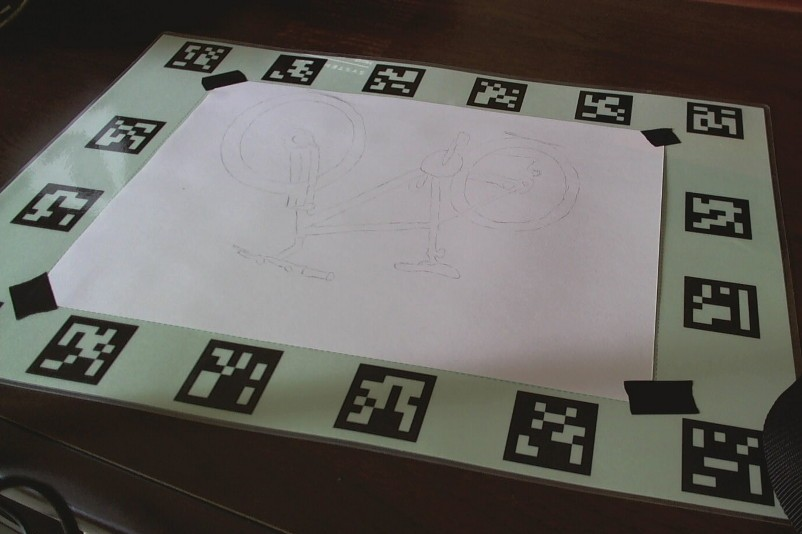
\includegraphics[height= 2.65cm]{cam}
                \caption{Webcam view.}
                \label{fig:webcam}
        \end{subfigure}
        \\
        \begin{subfigure}[b]{0.20\textwidth}
                \centering
                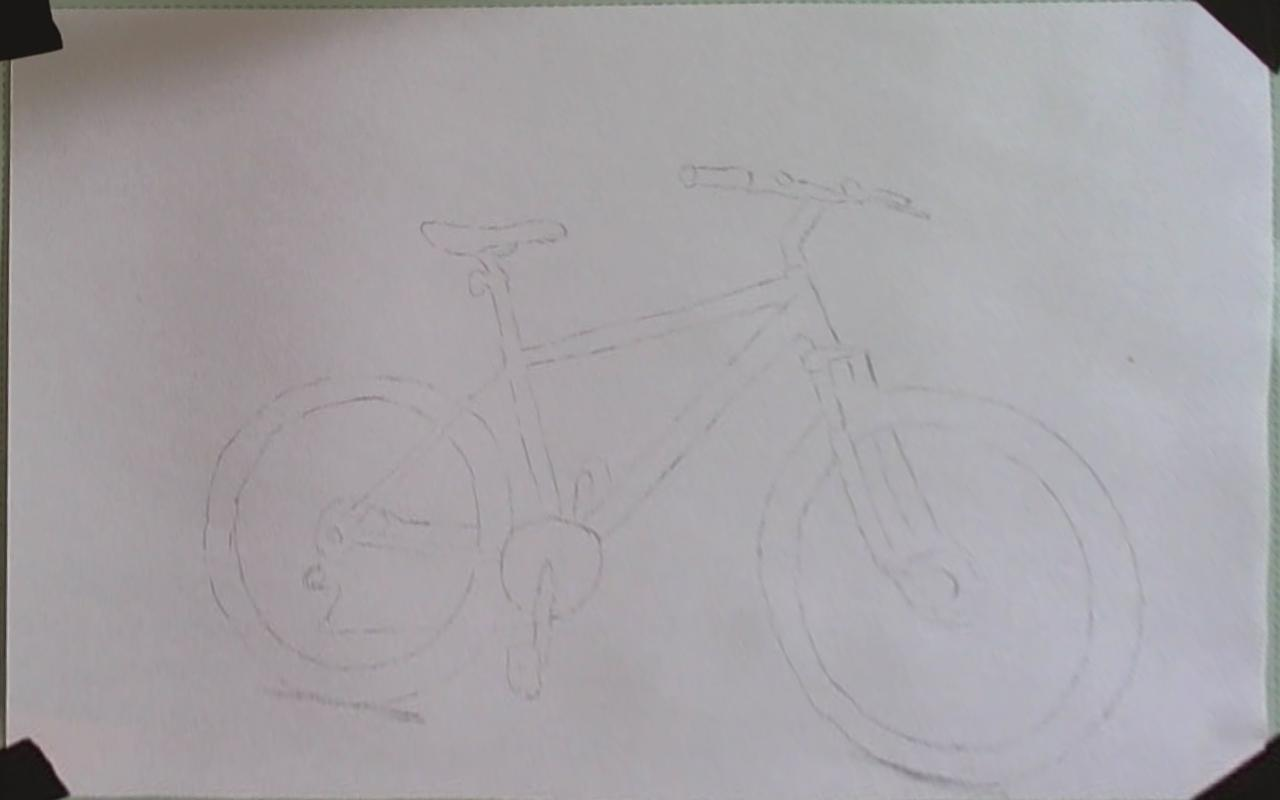
\includegraphics[height= 2.6cm]{extract}
                \caption{Drawing after extraction.}
                \label{fig:extract}
        \end{subfigure}
        ~ \hspace{4mm}
        \begin{subfigure}[b]{0.20\textwidth}
                \centering
                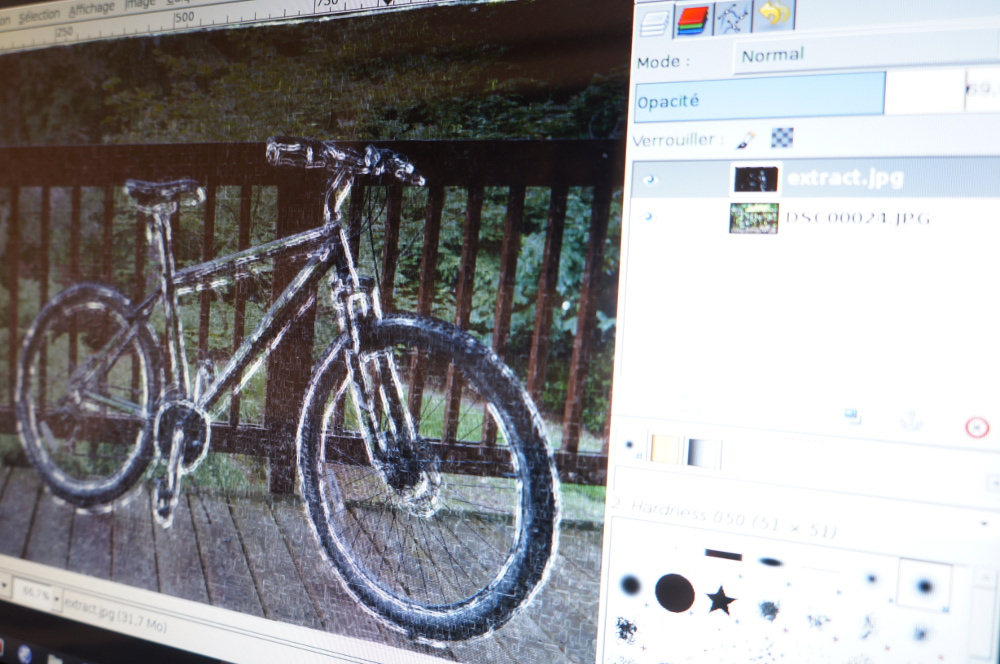
\includegraphics[height= 2.6cm]{DSC00286}
                \caption{Image edition software}
                \label{fig:gimp1}
        \end{subfigure}
        \\
        \begin{subfigure}[b]{0.20\textwidth}
                \centering
                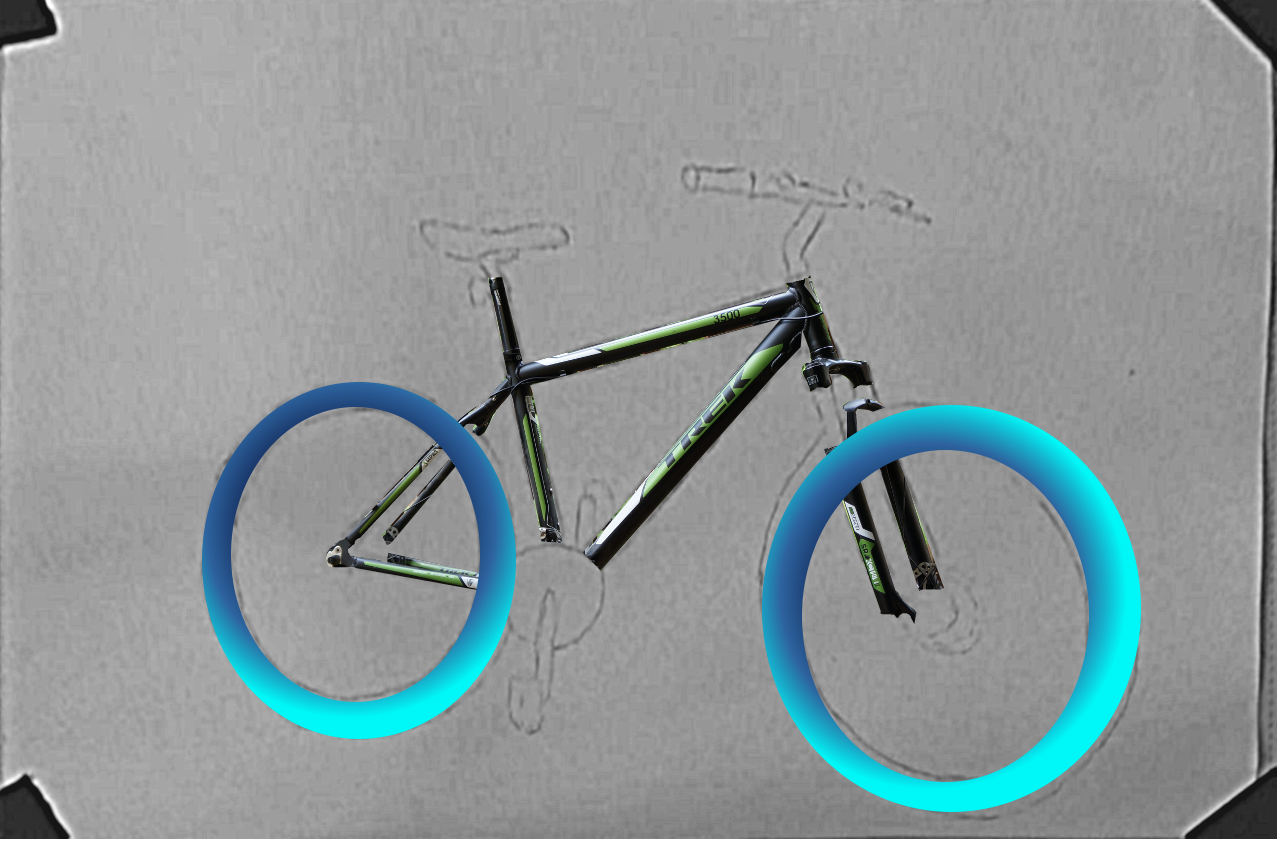
\includegraphics[height= 2.8cm]{mix2}
                \caption{Composition: preview}
                \label{fig:gimp2}
        \end{subfigure}
        ~ \hspace{4mm}
        \begin{subfigure}[b]{0.20\textwidth}
                \centering
                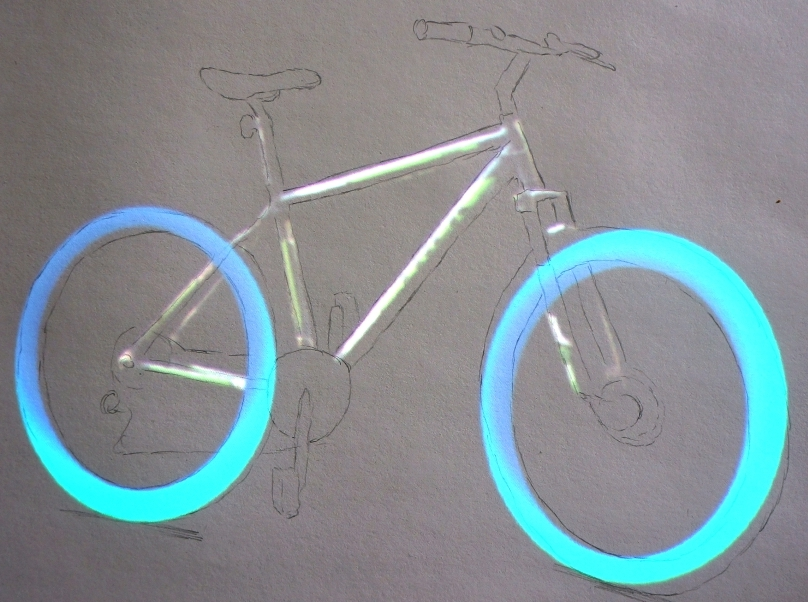
\includegraphics[height= 2.8cm]{velo2}
                \caption{Composition: photo}
                \label{fig:proj}
        \end{subfigure}
        \caption{From a photo (a), the user draws a first sketch captured by a webcam (b)(c); which is integrated as a layer in an image edition software (d)(e). Only the desired elements are projected (f) to continue the drawing if desired.}\label{fig:velo6illu}
\end{figure}


\section{Extensions}

An interesting extension would be to add color calibration between the physical tools and the projection. Using this, we would be able to simulate the output from a specific coloured pen or paint. Different pressure, or type of application could be calibrated and imported into the edition software. This way the artist could try appearances with various quantities of paint, or different pressures on a pen. However, this kind of feature promises future drawings, but the realisation will still be made by the artist; consequently adding some uncertainty and uniqueness on the result. 

On one hand, it would be useful to integrate our tool as a plug-in into the existing image edition software; providing a unique user interface. On the other hand, one could port the user interface of the image edition software in SAR. Considering the size and complexity of the current image edition software, it is challenging problem. Moreover, the use of tangible interface as we proposed in~\cite{laviole:2012} seems adapted, and may provide a whole experience of the drawing software. 

In this paper, we propose to extend drawing software, though the artist does not always creates drawings as a final result. It is possible to extend this for animation: the creation of digital tools for traditional animation would be a challenging task.  


\begin{figure}[!tb]
\centering
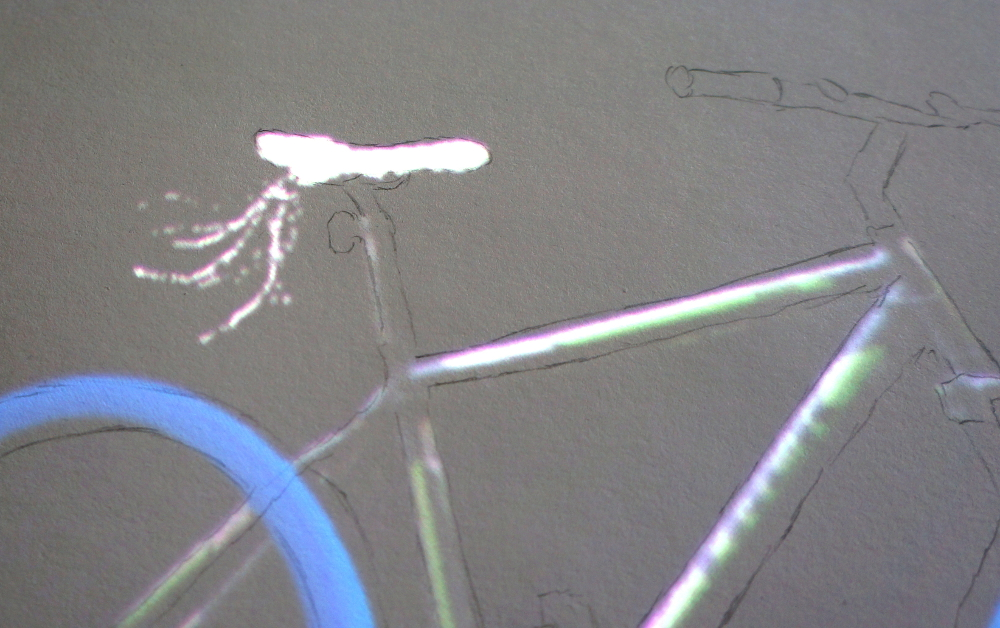
\includegraphics[width = 80mm]{velo4.JPG}
\caption{Closer view of the drawing plus projection. \vspace{-0.3cm}} 
\label{fig:zoom}
\end{figure}

\section{Conclusion}

In this paper we proposed spatial augmented reality (SAR) tools which merges physical drawing and digital drawing software. It allows a semi-automatic transfer between the physical drawing to the drawing software and vice versa. Our low-cost SAR solution allows any kind of drawing or painting and is non-intrusive. Furthermore, any image edition software can be used, and the example we provided is simple illustration of our system. We look forward to test this tool with professional artist who will find many more uses to our system, and may provide a valuable feedback on their desires for new SAR tools for physical drawings.


\bibliographystyle{abbrv}
\bibliography{paper}


\end{document}
